\documentclass[pdf,slideColor,frames,colorBG,accumulate,nototal]{prosper}
\usepackage{amsmath, amsfonts, amsbsy, pstricks, pst-node, pst-text, pst-3d}

\newcommand{\items}[1]{\begin{itemize} \item #1 \end{itemize}}
\newcommand{\itemss}[2]{\begin{itemize} \item #1 \item #2 \end{itemize}}
\newcommand{\itemsss}[3]{\begin{itemize} \item #1 \item #2 \item #3 \end{itemize}}
\newcommand{\itemssss}[4]{\begin{itemize} \item #1 \item #2 \item #3 \item #4
\end{itemize}}
\newcommand{\slidetextsize}{\footnotesize}
\newcommand{\captionstyle}[1]{\scriptsize \textbf{#1}}

% \myitem{1}{\includegraphics[width=.4cm]{red-bullet-on-blue}}
% \myitem{2}{\includegraphics[width=.4cm]{green-bullet-on-blue}}
% \myitem{3}{\includegraphics[width=.4cm]{yellow-bullet-on-blue}}

\newlength{\MiniPageLeft}
\newlength{\MiniPageRight}
\newlength{\ThisFigureWidth}

\title{Hybrid Orthogonal Genetic Algorithm for Global Numeric Optimization}
\author{Peter A. Stubberud and Matthew E. Jackson}
\email{stubber@ee.unlv.edu}
\institution{Department of Electrical and Computer Engineering, University of
Nevada - Las Vegas}
\Logo(10.,7.9){
\includegraphics[scale=0.35]{redlogo}}
\DefaultTransition{Box}

\DeclareSymbolFontAlphabet{\mathcalold}{symbols}
\newcommand{\mc}[1]{{\ensuremath{\mathcal{#1}}}}
\newcommand{\mco}[1]{{\ensuremath{\mathcalold{#1}}}}
\newcommand{\mr}[1]{{\ensuremath{\mathrm{#1}}}}
\newcommand{\mb}[1]{{\ensuremath{\mathbf{#1}}}}
\newcommand{\bs}[1]{\ensuremath{\boldsymbol{#1}}}
\newcommand{\ie}{\emph{i.e.}}
\newcommand{\Bayes}{Bayes's}
\newcommand{\field}[1]{\mathbb{#1}}
\newcommand{\real}[1]{\ensuremath{{\field{R}}^{#1}}}
\newcommand{\ints}[1]{\ensuremath{{\field{Z}}^{#1}}}
\newcommand{\defas}{\ensuremath{\stackrel{\scriptscriptstyle{\triangle}}{=}}}
\newcommand{\eye}[1]{\mr I_{#1}}
\newcommand{\model}{\mco I}
\newcommand{\pdf}[2][p]{\ensuremath{#1\left(#2\right)}}
\newcommand{\cpdf}[3][p]{\ensuremath{\pdf[#1]{\left.#2\,\right|\,#3}}}
\newcommand{\norm}[3]{\ensuremath{\mco N\left(#1\,\big|\,#2,\,#3\right)}}
\newcommand{\simnorm}[2]{\ensuremath{\sim \mco N\left(#1,\,#2\right)}}
\newcommand{\simIG}[2]{\ensuremath{\sim \mco{IG}\left(#1,\,#2\right)}}
\newcommand{\BSAR}[1]{\ensuremath{\text{BSAR}(#1)}}
\newcommand{\conv}{\ensuremath{\star}}

\begin{document}
\maketitle

\part{Go to full-screen mode now by hitting CTRL-L}

\begin{slide}{Introduction to Blind Deconvolution}
\slidetextsize
\begin{itemize}
\item Blind deconvolution fundamental in signal processing

\item Observation, $\mb x = \{x(t),\,t\in\mc T\}$, modelled as the convolution of unknown
source, $\{s(t),\,t\in\mc T\}$, with unknown distortion operator, $\mc A$; \ie\ $x(t)
\defas s(t) \conv\ \mc A$
\begin{figure}[t]
\begin{center}
        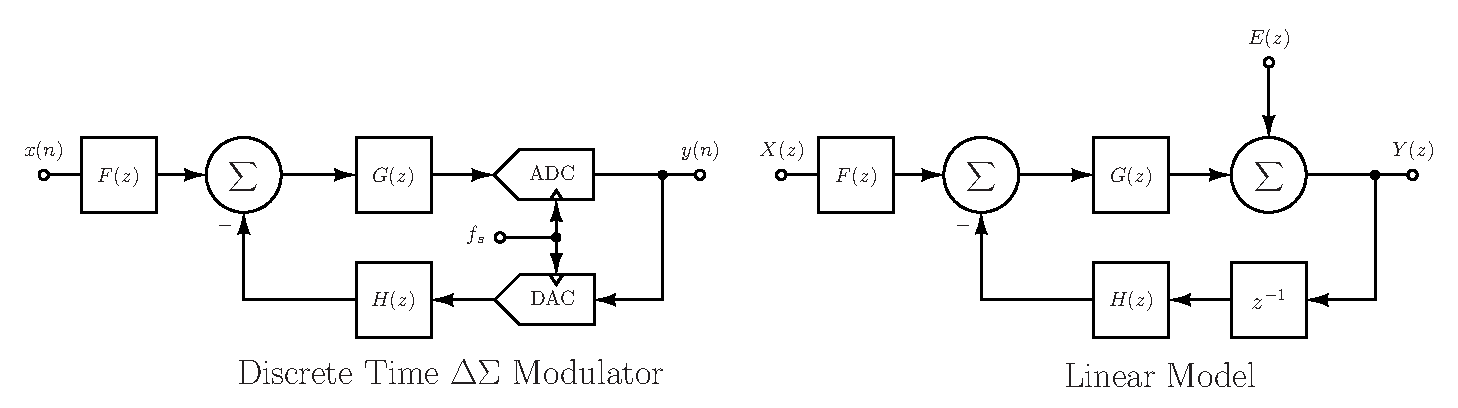
\includegraphics[width=\textwidth]{make_fig_final}
\end{center}
\end{figure}
\item Estimate $\mc A$, \emph{or} $\hat s(t) = a\,s(t - \tau)$, a scaled shifted version
of $s(t)$, where $a,\,\tau\in\real{}$, given only the observations, $\mb x$
\end{itemize}
\end{slide}

\begin{slide}{Equation Sheet 1}
\slidetextsize

 \begin{equation*}
  \text{STF}(z)=\frac{F(z)G(z)}{1+z^{-1}G(z)H(z)}\quad
  \text{NTF}=\frac{1}{1+z^{-1}G(z)H(z)}
 \end{equation*}
\end{slide}


\end{document}
